\documentclass[11pt,a4paper]{article}
\usepackage[margin=2.3cm]{geometry}
\usepackage[T1]{fontenc}
\usepackage{textcomp}
\input{glyphtounicode}
\pdfgentounicode=1
\usepackage{lmodern}
\usepackage{xcolor}
\usepackage{listings}
\usepackage{tcolorbox}
\usepackage{booktabs}
\usepackage{tikz}
\usepackage{hyperref}
\hypersetup{colorlinks=true, linkcolor=blue!50!black, citecolor=green!40!black}

\definecolor{codebg}{RGB}{248,248,245}
\lstset{
  language=C, basicstyle=\ttfamily\footnotesize, backgroundcolor=\color{codebg},
  keywordstyle=\color{blue!60!black}\bfseries, commentstyle=\color{green!45!black}\itshape,
  stringstyle=\color{red!60!black}, numbers=none, upquote=true,
  frame=single, rulecolor=\color{gray!40}, breaklines=true, columns=fullflexible,
  keepspaces=true, showstringspaces=false
}
\lstdefinestyle{sh}{language=bash, backgroundcolor=\color{black!5}}

\newtcolorbox{keyidea}{colback=blue!4, colframe=blue!45!black, title=Key ideas, fonttitle=\bfseries\small}
\newtcolorbox{experiment}{colback=orange!5, colframe=orange!70!black, title=Experiment, fonttitle=\bfseries\small}

\title{\textbf{OpenMP --- Lesson 2}\\[4pt]\large Shared vs.\ private variables, and the data race}
\author{Study notes for Flor Vargas}
\date{November 2026}

\begin{document}
\maketitle

\noindent\textit{\small Sources: Chapman, Jost \& van der Pas~\cite{chapman}, Ch.~4
``OpenMP Language Features'' (the \texttt{shared} and \texttt{private} clauses) and
Ch.~7 ``Troubleshooting'' (data races).}

\section{The idea}
All threads of a team live in the \textbf{same address space}. That is what
``shared-memory'' programming means. So for every variable used inside a parallel region,
we must know: is there \emph{one} copy that all threads use (\textbf{shared}), or does each
thread get \emph{its own} copy (\textbf{private})?

\begin{center}
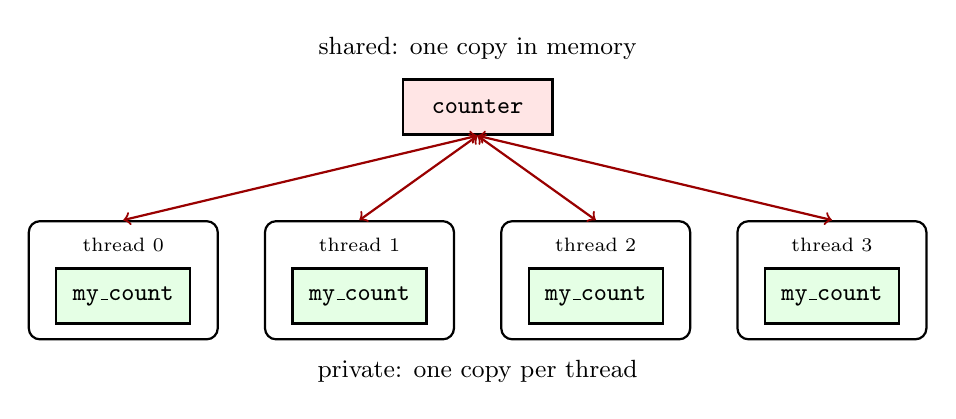
\begin{tikzpicture}[thick, box/.style={draw, minimum width=1.9cm, minimum height=0.7cm, font=\small\ttfamily}]
  \node[box, fill=red!10] (c) at (4.5,2.2) {counter};
  \node[font=\small] at (4.5,2.95) {shared: one copy in memory};
  \foreach \i/\x in {0/0,1/3,2/6,3/9} {
    \node[draw, rounded corners, minimum width=2.4cm, minimum height=1.5cm] (t\i) at (\x,0) {};
    \node[font=\scriptsize] at (\x,0.45) {thread \i};
    \node[box, fill=green!10, minimum width=1.7cm] at (\x,-0.2) {my\_count};
    \draw[<->, red!60!black] (t\i.north) -- (c.south);
  }
  \node[font=\small] at (4.5,-1.15) {private: one copy per thread};
\end{tikzpicture}
\end{center}

\section{The rules}
\begin{center}
\begin{tabular}{@{}ll@{}}
\toprule
Variable & Default attribute \\ \midrule
declared \emph{before} the parallel region & \textbf{shared} \\
declared \emph{inside} the region (incl.\ a \texttt{for} loop index declared there) & \textbf{private} \\
listed in a \texttt{private(\ldots)} clause & \textbf{private}, new \emph{uninitialised} copy \\
listed in a \texttt{shared(\ldots)} clause & \textbf{shared} (makes the default explicit) \\
\bottomrule
\end{tabular}
\end{center}

\section{The data race}
\texttt{counter++} looks like one operation but the CPU does three: \emph{read}
\texttt{counter} into a register, \emph{add} 1, \emph{write} it back. If two threads read
the same old value before either writes, both write the same new value, and one increment
is lost:
\begin{center}
\begin{tabular}{@{}lll@{}}
\toprule
time & thread 0 & thread 1 \\ \midrule
1 & read \texttt{counter} $\to$ 5 & \\
2 & & read \texttt{counter} $\to$ 5 \\
3 & write 6 & \\
4 & & write 6 \quad (should be 7) \\
\bottomrule
\end{tabular}
\end{center}
This is a \textbf{data race}: two or more threads access the same memory location, at
least one of them writes, and nothing orders the accesses. The result depends on timing.

\section{The code}
\lstinputlisting[title=\texttt{shared\_private.c}]{shared_private.c}

\begin{lstlisting}[style=sh]
gcc -Wall -fopenmp -o shared_private shared_private.c
OMP_NUM_THREADS=4 ./shared_private
\end{lstlisting}
Typical output (your numbers will differ):
\begin{lstlisting}[style=sh]
  thread 1: my_count = 1000000
  thread 3: my_count = 1000000
  thread 0: my_count = 1000000
  thread 2: my_count = 1000000
expected counter = 4000000
actual   counter = 2297568
\end{lstlisting}

\begin{keyidea}
\begin{itemize}
  \item Every \texttt{my\_count} is exactly $10^6$: private data is always safe.
  \item \texttt{counter} is wrong and changes from run to run: a shared variable that
        several threads \emph{write} is a race unless something coordinates them.
  \item Reading shared data is fine. The problem is concurrent \emph{writes}.
  \item \texttt{private(x)} gives an uninitialised copy. Always assign it inside the region.
  \item \texttt{nthreads} is shared but written by only one thread, so there is no race.
\end{itemize}
\end{keyidea}

\section{The experiment}
\begin{experiment}
\textbf{Question:} when does the race appear, and is it reproducible?
\begin{enumerate}
  \item Run with 1, 2 and 4 threads:
\begin{lstlisting}[style=sh]
for t in 1 2 4; do echo "== $t threads"; OMP_NUM_THREADS=$t ./shared_private; done
\end{lstlisting}
  \item Run the 4-thread case five times and compare the last line:
\begin{lstlisting}[style=sh]
for r in 1 2 3 4 5; do OMP_NUM_THREADS=4 ./shared_private | tail -1; done
\end{lstlisting}
  \item Change \texttt{\#define N 1000000} to \texttt{\#define N 100}, recompile, and repeat
        step 2.
\end{enumerate}
\textbf{What to observe and answer.}
\begin{enumerate}
  \item Why is the result always correct with 1 thread?
  \item Why does the wrong value change between runs?
  \item With \texttt{N 100} the result is usually correct. Does that mean the program is
        correct?
\end{enumerate}
\end{experiment}

\paragraph{Answers (read after trying).}
(1)~With one thread there is nobody to race with: the read--add--write sequences never
interleave.
(2)~How often two threads interleave their read and write depends on scheduling and
timing, which change every run. This is why races are hard to debug.
(3)~No. With few iterations each thread finishes before the next one even starts, so the
accesses rarely overlap. The race is still there and can appear at any time. A program
that is ``usually right'' is wrong. Never trust a parallel result just because one test
passed.

\paragraph{Next lesson.} How to update a shared variable safely: \texttt{critical},
\texttt{atomic}, and the \texttt{reduction} clause, which is the right tool for this
counter (Chapman et al., Ch.~4).

\begin{thebibliography}{9}
\bibitem{chapman} B.~Chapman, G.~Jost, and R.~van der Pas. \emph{Using OpenMP: Portable
  Shared Memory Parallel Programming}. MIT Press, Cambridge, MA, 2007.
\end{thebibliography}
\end{document}
